\chapter{Результаты эксперимнетальных исследований мобильных водоплавающих роботов}\label{ch:ch4}

\section{Методика проведения эксмериментальных исследований}\label{sec:ch4/sec1}

\section{Экспериментальные исследования с водоплавающим мобильным роботом в форме эллипсоида}\label{sec:ch4/sec2}

Эксперименты проводились в бассейне размерами 3х1.5х1.5 м, заполненном водой. Цель экспериментов -- определение характера движения безвинтового подводного робота при различных управляющих воздействиях. В качестве управляющих воздействий выступают гиростатические моменты роторов K1, K2, K3, возникающие при их вращении. Рассмотрены три серии экспериментов: вращение только пары больших роторов, вращение только одной пары меньших роторов и одновременное вращение пары больших и одной пары меньших роторов. В каждом эксперименте роторы разгонялись до максимальной скорости 590 об/мин.

Так как роторы 2 и 3 имеют одинаковые массо-геометрические характеристики и лежат в одной плоскости, их совместное вращение приведет к качественно аналогичному, результату, что и в случае их вращения по отдельности.


1.	Вращение пары больших роторов. В качестве управляющего воздействия выступала угловая скорость пары больших роторов, ось вращения которых совпадает с большей полуосью эллипсоида. Роторы разгонялись до максимальной скорости 590 об/мин, которая поддерживалась постоянной в течение 3 секунд. Вектор внутреннего гиростатического момента, сообщенный телу после разгона роторов, $K = (2i_1\omega_{max}, 0, 0)$. Для данных управляющих воздействий была проведена серия из трех экспериментов. Результаты численного моделирования при вышеописанных управляющих воздействиях и результаты экспериментов представлены на рисунке \ref{Exp_BPR_1}.

\begin{figure}[ht]
	\centering
	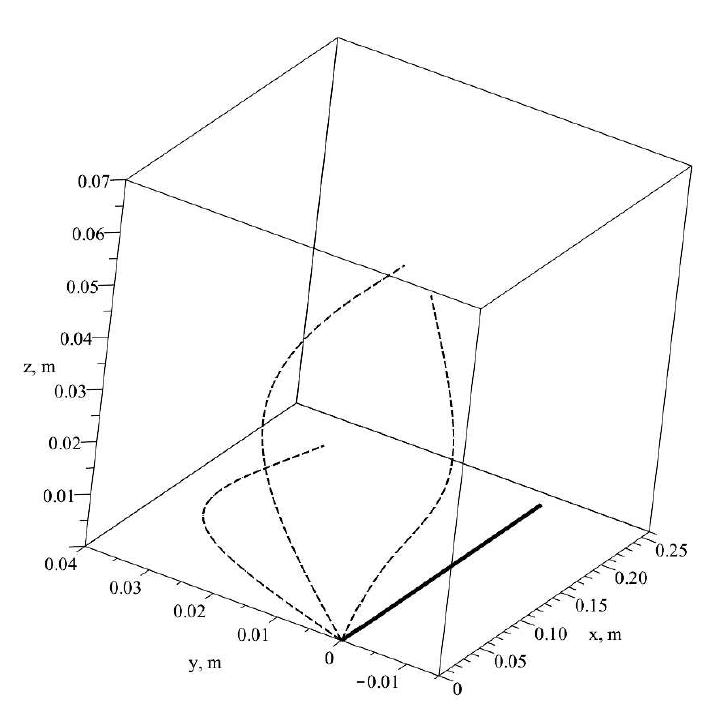
\includegraphics[width=0.5\linewidth]{Exp_BPR_1.png}%
	\caption{Теоретическая (сплошная линия) и экспериментальные (штриховые линии) траектории движения безвинтового подводного робота при $K = (2i_1\omega_{max}, 0, 0)$}
	\label{Exp_BPR_1}
\end{figure}


2.	Вращение одной пары малых роторов. В качестве управляющего воздействия выступала угловая скорость одной пары малых роторов. Роторы разгонялись до максимальной скорости 590 об/мин, которая поддерживалась постоянной в течение 3 секунд. Вектор гиростатического момента, сообщенный телу после разгона роторов, $K = (0, 2i_2\omega_{max}, 0)$. Для данных управляющих воздействий была проведена серия из трех экспериментов. Результаты численного моделирования при вышеописанных управляющих воздействиях и результаты экспериментов представлены на рисунке \ref{Exp_BPR_2}.

\begin{figure}[ht]
	\centering
	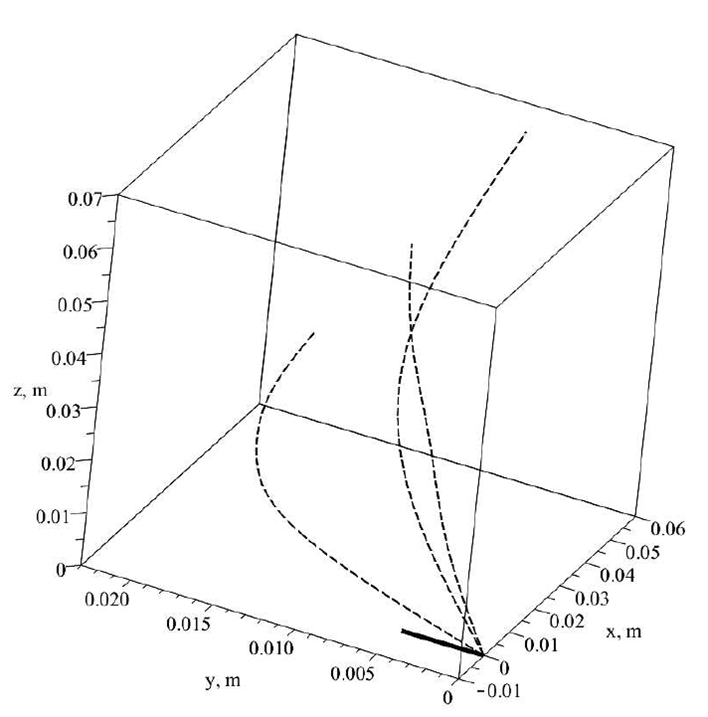
\includegraphics[width=0.5\linewidth]{Exp_BPR_2.png}%
	\caption{Теоретическая (сплошная линия) и экспериментальные (штриховые линии) траектории движения безвинтового подводного робота при $K = (0, 2i_2\omega_{max}, 0)$}
	\label{Exp_BPR_2}
\end{figure}


3.	Вращение пары больших роторов и одной пары малых роторов. В качестве управляющего воздействия выступала угловая скорость одной пары малых и пары больших роторов. Роторы разгонялись до максимальной скорости 590 об/мин, которая поддерживалась постоянной в течение 3 секунд. Вектор гиростатического момента, сообщенный телу после разгона роторов, $K = (2i_1\omega_{max}, 2i_2\omega_{max}, 0)$. Результаты численного моделирования при вышеописанных управляющих воздействиях и результаты экспериментов представлены на рисунке \ref{Exp_BPR_3}.

\begin{figure}[ht]
	\centering
	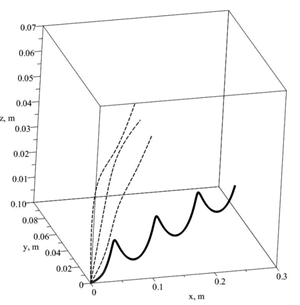
\includegraphics[width=0.5\linewidth]{Exp_BPR_3.png}%
	\caption{Теоретическая (сплошная линия) и экспериментальные (штриховые линии) траектории движения безвинтового подводного робота при $K = (2i_1\omega_{max}, 2i_2\omega_{max}, 0)$}
	\label{Exp_BPR_3}
\end{figure}

Несмотря на указанную теоретическую возможность перемещения подводного робота с помощью вращения роторов, экспериментальные данные существенно отличаются от результатов, полученных в рамках модели идеальной жидкости. Например, при первых двух вариантах управляющих воздействий в рамках теоретической модели робот движется прямолинейно не изменяя своей ориентации. При проведении экспериментов такого движения добиться не удается. Кроме того, перемещение безвинтового подводного робота на практике в два раза меньше теоретического.


\section{Экспериментальные исследования с водоплавающим недеформируемым рыбоподобным роботом}\label{sec:ch4/sec3}
	
	
\clearpage